As $Q^2$ is pushed higher, inelastic scattering begins to give way to DIS. In this kinematic region, the wavelength of the virtual photon is sufficiently short to resolve the internal structure of the nucleon. This transition sees the system begin to behave like a free Dirac particle, the parton. As the Bjorken limit is approached, $Q^2\rightarrow\infty$ and $\nu\rightarrow\infty$, the scattering center approaches a structureless parton.\cite{Bjorken_scaling} With this in mind, it is useful to look at the cross section for scattering off of a structureless target:

\begin{equation}
	\frac{d^2\sigma}{d\Omega dE^\prime} = \frac{\alpha^2}{4E^{2}\sin^{4}\frac{\theta}{2}} \left[\cos^{2}\frac{\theta}{2} + \frac{Q^2}{2m^2}\sin^{2}\frac{\theta}{2}\right] \delta\left(\nu-\frac{Q^2}{2M}\right)
	\label{xs_no_struct}
\end{equation}

Noting that DIS is scattering off of a structureless parton, we can compare (\ref{xs_inelastic}) and (\ref{xs_no_struct}). By equating these two cross sections, we can clearly extract equations for the DIS structure functions.

\begin{subequations}
\begin{align}
	2MW_1\left(Q^{2},\nu\right) = \frac{Q^2}{2M\nu}\delta\left(1-\frac{Q^2}{2M\nu}\right) \\
	\nu W_2\left(Q^{2},\nu\right) = \delta\left(1-\frac{Q^2}{2M\nu}\right)
\end{align}
\end{subequations}

In this kinematic region, we see that the structure functions are dependent on the ratio $\frac{Q^2}{2M\nu}$ rather than $Q^2$ and $\nu$ independently while the target mass sets the scale. Noting this dependency, the scaling variable Bjorken $x$ is defined as
\begin{equation}
	x = \frac{Q^2}{2M\nu}.
\end{equation}
As the Bjorken limit is approached DIS is only dependent on $x$, showing little to no scaling with $Q^2$ or $\nu$.\cite{bodek_scaling} New structure functions, $F_1$ and $F_2$, are also defined in terms of $x$ to clearly show the lack of scaling with $Q^2$ and $\nu$ independently:

\begin{subequations}
\begin{align}
	2MW_1\left(Q^{2},\nu\right) \rightarrow F_{1}\left(x\right) \\
	\nu W_2\left(Q^{2},\nu\right) \rightarrow F_{2}\left(x\right)
\end{align}
\label{eqn:w_to_f}
\end{subequations}

The independence of structure functions with respect to $Q^2$ has been experimentally tested. The data was taken at fixed $x$ with varying $Q^2$. All measurements were consistent with no $Q^2$ dependence. Proton data showing this effect for the structure function $F_2$ can be seen in Figure \ref{fig:noQ2F2}. Substituting Equations \ref{eqn:w_to_f} into Equation \ref{xs_inelastic} we find the cross section in terms of DIS $x$, Equation \ref{eqn:x_dis_xs}.

\begin{equation}
	\frac{d^2\sigma}{d\Omega dE^\prime} = \frac{4\alpha^2\left(E^\prime\right)^2}{Q^4}\cos^2\left(\frac{\theta}{2}\right) \left[\frac{F_2\left(x\right)}{\nu} + \frac{2F_1\left(x\right)}{M}\tan^2\left(\frac{\theta}{2}\right)\right]
	\label{eqn:x_dis_xs}
\end{equation}

\begin{figure}
\begin{center}
	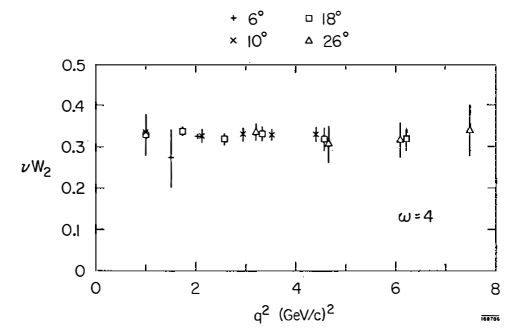
\includegraphics[width=0.75\textwidth]{./scattering/fig/no_q2_dep.png}
	\caption{Proton data showing no $Q^2$ dependence of $\nu W_2=F_2$ in the DIS region.\cite{FriedmanKendall}}
	\label{fig:noQ2F2}
\end{center}
\end{figure}